\documentclass[9pt,a4paper,twoside]{template/document}
%\usepackage[english]{babel}

%% Spanish babel recomendation
\usepackage[spanish,es-nodecimaldot,es-noindentfirst]{babel}
\usepackage{amsmath}
\usepackage{longtable}

%----------------------------------------------------------
% Title
%----------------------------------------------------------

\doctype{Arquitectura del Software (TB034)}
\title{Trabajo Práctico 1}
\logo{logo}

%----------------------------------------------------------
% Authors, Affiliations and dates
%----------------------------------------------------------

\author[]{
    Sebastian Vintoñuke -- 106063             \newline
    Cindy Teresa Hsieh -- 108051              \newline
    Maria Delfina Cano Ros Langrehr -- 109338 \newline
    Lautaro Martin Sotelo -- 107472
}

%----------------------------------------------------------

%\affil[1]{UBA | Facultad de Ingeniería}

%----------------------------------------------------------

%\dates{This manuscript was compile on February 24, 2026}

%----------------------------------------------------------
% Corresponding author-, Document- information
%----------------------------------------------------------

%\corres{\textsuperscript{\textasteriskcentered}Corresponding author: \href{mailto:author.one@institute.org}{author.one@institute.org} (A. One).}
%\corres{\textsuperscript{\textdagger}These authors contributed equally to this work.}

%----------------------------------------------------------

%\docinfo{This document class was prepared on Overleaf and compiled with pdf\LaTeX{}. No errors were found during the compilation process. This class supports external editors, though additional setup may be required.}

%----------------------------------------------------------

\journalname{UBA | Facultad de Ingeniería}
\footerlogo{logo\_fiuba\_big}
\journal{Arquitectura del Software (TB034)}
\theday{\today}
%\vol{}
%\no{}

%----------------------------------------------------------
% Abstract y palabras clave
% (opcional: se arma con \abstracttitle{...} + \begin{abstract}...\end{abstract};
% si no se definen, la caja del abstract no se dibuja)
%----------------------------------------------------------

%----------------------------------------------------------

%\keywords{Document Class, Research Article, Laboratory Report, Academic Writing, Journal}

%----------------------------------------------------------

\begin{document}

\maketitle
\thispagestyle{firststyle}

%----------------------------------------------------------

% TODO: BORRAR PARA LA ENTREGA
\newcommand{\recordatorioevidencia}{
    \begin{tcolorbox}[
        colback=red!10,
        colframe=red!80!black,
        boxrule=1pt,
        arc=2mm
    ]
    \textbf{Toda} afirmación que se realice debe estar apoyada en \textbf{evidencia}.
    Si se encuentra alguna \textbf{afirmación} que no está correctamente \textbf{fundamentada}
    con \textbf{evidencia}, se disminuirá la nota. Esto incluye las observaciones que
    realicen sobre el código y su funcionamiento en general. Que no existan
    métricas para un determinado QA no implica que no pueda evidenciarse el
    efecto de una táctica.
    \end{tcolorbox}
}
\recordatorioevidencia

% TODO bloque de comentarios, sacar al final
\newcommand{\todo}[1]{\vspace{2mm}\noindent\colorbox{yellow}{\textbf{TODO:}}\colorbox{yellow!20}{\parbox[t]{0.9\textwidth}{#1}}\vspace{2mm}}

\section{Sistema Recibido}
\label{sec:sistema_recibido}

    \begin{figure}[H]
        \centering
        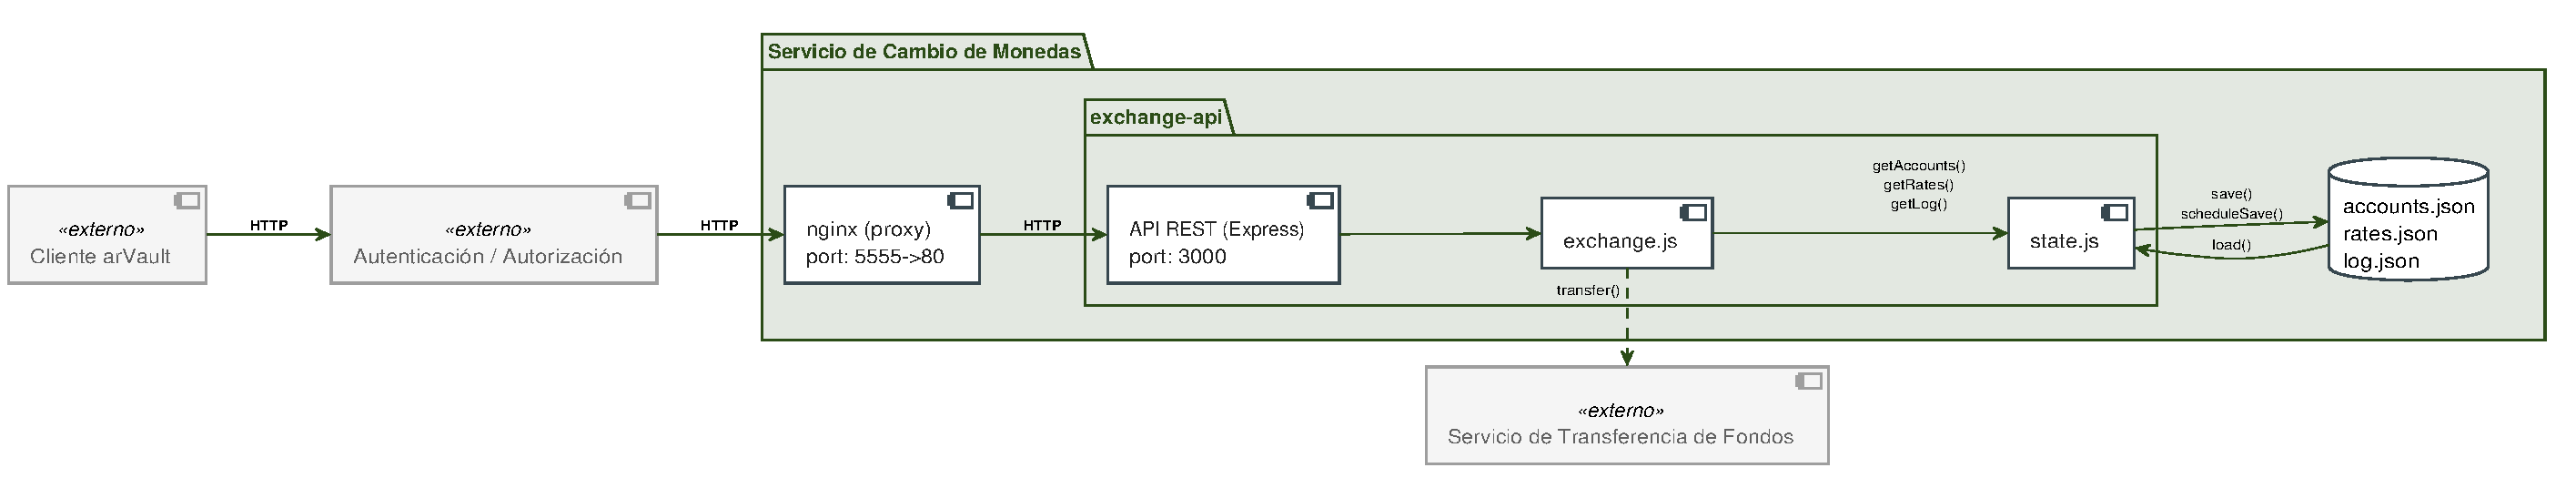
\includegraphics[width=1\columnwidth]{figures/componentes_y_conectores_base}
        \caption{ Diagrama Components \& Connectors del sistema base. }
        \label{fig:componentes_y_conectores_base}
    \end{figure}

    \subsection{Arquitectura}
    \label{sec:arquitectura}

    El despliegue recibido sigue una arquitectura cliente-servidor. Nginx actúa como
    reverse proxy y deriva las solicitudes hacia una única instancia de la API de
    intercambio implementada con Node.js y Express. El despliegue también incluye
    Graphite/StatsD, Grafana y cAdvisor como componentes de observabilidad, aunque
    estos no forman parte de la lógica de negocio.

    Dentro de la API existe una separación lógica en tres módulos: \texttt{app.js}
    expone la interfaz HTTP, \texttt{exchange.js} coordina las operaciones de cambio
    y \texttt{state.js} carga y persiste el estado. Esta separación es parcial: la
    lógica de negocio conserva referencias mutables a cuentas, tasas y logs, y
    modifica directamente dichas estructuras.

    El archivo \texttt{docker-compose.yml} declara una sola instancia de la API y no
    configura réplicas, health checks ni una política de reinicio. Por lo tanto, una
    caída del proceso interrumpe el servicio hasta que un operador o una herramienta
    externa lo vuelva a iniciar. Además, la API es stateful: mantiene las cuentas,
    tasas y operaciones en memoria, por lo que agregar réplicas sin introducir un
    mecanismo de coordinación produciría estados divergentes.

    La persistencia se realiza periódicamente sobre archivos JSON. Las cuentas y el
    log se escriben cada segundo, mientras que las tasas se escriben cada cinco
    segundos. En consecuencia, existe una ventana entre la modificación en memoria
    y su escritura en disco durante la cual una terminación abrupta puede provocar
    pérdida de datos. Esto no constituye un protocolo de consistencia eventual, sino
    una estrategia de durabilidad diferida sin garantías transaccionales.

    \subsection{Código}
    \label{sec:codigo}

    La separación de responsabilidades es incompleta. \texttt{exchange.js} calcula
    importes, coordina las llamadas al servicio de transferencias, valida el saldo
    interno, modifica las cuentas y registra el resultado. Esta concentración aumenta
    el acoplamiento y dificulta probar cada responsabilidad de forma aislada.

    \begin{code}
        \lstinputlisting[language=JavaScript]{./code/exchange_method.js}
        \caption{app/exchange.js}
        \label{lst:separacion_de_responsabilidades}
    \end{code}

    \texttt{state.js} no expone directamente sus variables internas, pero sus getters
    retornan las mismas referencias mutables almacenadas por el módulo. Luego de la
    inicialización, \texttt{exchange.js} conserva esas referencias y modifica los
    objetos sin pasar por una operación explícita del componente de persistencia.
    Por ello, la abstracción es permeable: reemplazar los JSON por un repositorio o
    una base de datos requeriría adaptar también la forma en que la lógica de negocio
    lee y actualiza el estado.

    \begin{code}
        \lstinputlisting[language=JavaScript]{./code/acoplamiento.js}
        \caption{app/exchange.js}
        \label{lst:acoplamiento}
    \end{code}

    El endpoint de cambio también contiene una condición de carrera. La comprobación
    de saldo se ejecuta antes de dos operaciones asíncronas. Mientras una solicitud se
    encuentra suspendida en un \texttt{await}, otra puede comprobar el mismo saldo y
    aprobar la operación. Ambas solicitudes pueden completar los descuentos y dejar
    un saldo negativo. El Listado~\ref{lst:race_condition} muestra la sección crítica,
    que no está protegida por exclusión mutua, serialización ni una transacción.

    \begin{code}
        \lstinputlisting[language=JavaScript]{./code/race_condition.js}
        \caption{Sección crítica de \texttt{app/exchange.js} en el caso base.}
        \label{lst:race_condition}
    \end{code}

    El registro de operaciones tampoco tiene una política de retención. Cada resultado
    se agrega a un arreglo en memoria y \texttt{GET /log} devuelve el arreglo completo.
    A medida que aumenta la cantidad de operaciones, crecen el consumo de memoria, el
    tamaño de la respuesta y el trabajo necesario para serializar el estado. Además,
    el arreglo completo se convierte a JSON y se reescribe cada segundo, por lo que el
    costo de cada persistencia aumenta con el historial.

    \begin{code}
        \lstinputlisting[language=JavaScript]{./code/log_growth.js}
        \caption{Crecimiento y persistencia del log en el caso base.}
        \label{lst:log_growth}
    \end{code}

    La escritura utiliza directamente el archivo definitivo. No se escribe primero a
    un archivo temporal ni se realiza un reemplazo atómico, por lo que una interrupción
    durante \texttt{writeFile} puede dejar un JSON incompleto. El manejo de errores de
    \texttt{state.js} registra el fallo, pero no lo propaga ni permite que la API informe
    que el estado no pudo persistirse.

    \begin{code}
        \lstinputlisting[language=JavaScript]{./code/save.js}
        \caption{app/state.js}
        \label{lst:save}
    \end{code}

    Los importes monetarios se representan mediante \texttt{Number}, cuyo formato de
    punto flotante binario no representa exactamente todos los valores decimales. Sin
    una regla explícita de redondeo o una representación en unidades mínimas, el error
    puede acumularse en los saldos y en los importes entregados al cliente.

    \begin{code}
        \lstinputlisting[language=JavaScript]{./code/floats.js}
        \caption{Cálculo monetario con \texttt{Number} en \texttt{app/exchange.js}.}
        \label{lst:floats}
    \end{code}

    Finalmente, las validaciones HTTP comprueban únicamente la presencia mediante
    condiciones de truthiness. No se validan tipos, rangos, monedas soportadas ni
    coherencia entre moneda y cuenta. Por ejemplo, un importe negativo supera la
    validación inicial y puede alterar los saldos en el sentido contrario al esperado.
    Las monedas inexistentes también pueden producir excepciones al acceder a una tasa
    o cuenta no encontrada. A su vez, los rechazos de negocio se informan como HTTP 500,
    aunque no necesariamente representan una falla interna del servidor.

    \begin{code}
        \lstinputlisting[language=JavaScript]{./code/request_validation.js}
        \caption{Validación por presencia en \texttt{app/app.js}.}
        \label{lst:request_validation}
    \end{code}

    \begingroup
    \small
    \setlength{\tabcolsep}{4pt}
    \renewcommand{\arraystretch}{1.2}
    \begin{longtable}{@{}p{0.13\textwidth}p{0.22\textwidth}p{0.12\textwidth}p{0.19\textwidth}p{0.19\textwidth}@{}}
        \caption{Hallazgos del análisis estático del caso base.}
        \label{tab:hallazgos_codigo_base}\\
        \toprule
        \textbf{Hallazgo} & \textbf{Evidencia} & \textbf{QA afectados} & \textbf{Consecuencia posible} & \textbf{Validación propuesta} \\
        \midrule
        \endfirsthead
        \toprule
        \textbf{Hallazgo} & \textbf{Evidencia} & \textbf{QA afectados} & \textbf{Consecuencia posible} & \textbf{Validación propuesta} \\
        \midrule
        \endhead
        Carrera concurrente & La verificación de saldo precede a dos operaciones asíncronas y el descuento ocurre después (Listado~\ref{lst:race_condition}). & Reliability, Security & Dos solicitudes pueden aprobarse con el mismo saldo y producir un balance negativo. & Ejecutar dos cambios concurrentes de 80 unidades contra un saldo interno de 100 y observar respuestas y saldo final. \\
        \midrule
        Estado mutable expuesto & Los getters de \texttt{state.js} retornan objetos que \texttt{exchange.js} conserva y modifica. & Modificabilidad, Testability, Reliability & Las actualizaciones eluden una interfaz de repositorio y dificultan sustituir o simular la persistencia. & Probar la lógica con un repositorio simulado y registrar qué dependencias deben reemplazarse. \\
        \midrule
        Log sin límite & Cada operación ejecuta \texttt{log.push}; \texttt{GET /log} retorna el arreglo completo (Listado~\ref{lst:log_growth}). & Performance, Scalability, Availability & Aumentan memoria, tamaño de respuesta y tiempo de serialización con cada operación. & Ejecutar lotes crecientes y medir memoria, bytes y latencia de \texttt{GET /log}. \\
        \midrule
        Reescritura completa & \texttt{scheduleSave} serializa y escribe el log completo cada segundo. & Performance, Efficiency, Reliability & El costo de I/O crece con el historial y una interrupción puede dejar el archivo incompleto. & Medir tamaño, tiempo de escritura y actividad de I/O para distintos volúmenes de log. \\
        \midrule
        Durabilidad diferida & Los cambios residen en memoria hasta el siguiente intervalo y la escritura no es atómica. & Reliability, Availability & Una terminación abrupta puede perder operaciones confirmadas o impedir cargar el JSON. & Terminar la API dentro de la ventana de persistencia, reiniciarla y comparar estado y log. \\
        \midrule
        Dinero con \texttt{Number} & El importe se obtiene mediante \texttt{baseAmount * exchangeRate} sin redondeo explícito (Listado~\ref{lst:floats}). & Reliability, Security & Pueden aparecer residuos decimales y acumularse diferencias en los saldos. & Utilizar valores como 0.1 y 0.2 y comparar contra un cálculo decimal exacto. \\
        \midrule
        Validación incompleta & La API solo verifica truthiness y acepta valores negativos o combinaciones incoherentes (Listado~\ref{lst:request_validation}). & Security, Reliability, Testability & Entradas inválidas pueden alterar saldos o provocar excepciones no controladas. & Crear casos con importes negativos, tipos incorrectos, monedas inexistentes y cuentas incompatibles. \\
        \bottomrule
    \end{longtable}
    \endgroup

    \subsection{Infraestructura}
    \label{sec:infraestructura}

    La infraestructura se define mediante Docker Compose. Nginx publica la API en el
    puerto 5555; Grafana, Graphite/StatsD y cAdvisor conforman el subsistema de
    observabilidad. La API no publica directamente su puerto al host, por lo que las
    pruebas externas deben atravesar Nginx, tal como requiere el enunciado.

    El estado de la API se copia dentro de la imagen y no está asociado a un volumen.
    Por lo tanto, eliminar o recrear el contenedor descarta las modificaciones de sus
    archivos JSON. Grafana sí utiliza un volumen, mientras que Graphite no declara uno
    para conservar sus series. Estas decisiones limitan la durabilidad y la
    reproducibilidad de las mediciones entre recreaciones del entorno.

    \todo{Agregar evidencia de ejecución sobre recuperación, persistencia y funcionamiento de cAdvisor en el equipo de pruebas.}

\section{Atributos de calidad}
\label{sec:atributos_de_calidad}

    \subsection{Identificación de los QA claves}
    \label{sec:identificacion_de_los_qa_claves}

        Se identifican los siguientes atributos de calidad como claves en el contexto del negocio.
        Adicionalmente, se citan especificaciones y requerimientos que motivaron estas afirmaciones.

        \subsubsection{Availability (disponibilidad)}
        \label{sec:disponibilidad}

            Habilidad del sistema para reparar o enmascarar fallas de manera tal que el período fuera de servicio no exceda un determinado valor durante un lapso de tiempo especificado.

            \begin{customenv}[frametitle=]
                La startup arVault es una fintech que opera una billetera digital
            \end{customenv}

            Al ser una billetera digital, el servicio permite manipular el dinero de los usuarios. Un servicio con baja o nula disponibilidad implicaria que los usuarios no pueden acceder a su propio dinero.
            Adicionalmente, el modelo de negocio se basa en que los usuarios operen, si el servicio no es disponible para permitir estas operaciones, se estan perdiendo potenciales ganancias.

        \subsubsection{Performance}
        \label{sec:performance}

            Habilidad del sistema para reaccionar ante ciertos eventos en un determinado tiempo.

            \begin{customenv}[frametitle=]
                Si bien el lanzamiento fue exitoso, comenzaron a aparecer reclamos de los usuarios sobre problemas en el uso de la función de cambio de monedas.
            \end{customenv}

            Uno de los principales candidatos a explicar los reclamos es el endpoint
            \texttt{/exchange}. Una operación exitosa realiza dos transferencias
            secuenciales de entre 200 y 400 milisegundos cada una, por lo que su tiempo
            de respuesta esperado es mayor que el de los endpoints que solo consultan
            memoria. Esta hipótesis debe contrastarse con las pruebas de carga.

            \begin{customenv}[frametitle=]
                las tasas de cambio no tienen gap entre el valor de compra y de venta.
            \end{customenv}

            La ausencia de gap significa que la compra y la venta utilizan la misma
            cotización; no implica por sí misma que la tasa se actualice en tiempo real.
            Sin embargo, una latencia elevada aumenta el tiempo entre la cotización y
            la finalización del cambio, y por ello incrementa el riesgo de operar con
            un valor que ya no represente las condiciones vigentes.

        \subsubsection{Scalability (escalabilidad)}
        \label{sec:escalabilidad}

            Habilidad del sistema para incorporar recursos adicionales de manera efectiva. Efectividad = mejora mensurable de algún QA + no requerir un esfuerzo inapropiado + no interrumpir el funcionamiento.

            \begin{customenv}[frametitle=]
                Para ganar usuarios, las tasas de cambio...
            \end{customenv}

            Se especifica que el objetivo a corto plazo es incrementar el número de
            usuarios. El sistema debe poder acompañar ese crecimiento incorporando
            recursos sin interrumpir el servicio ni exigir un esfuerzo inapropiado.

        \subsubsection{Reliability (confiabilidad)}
        \label{sec:confiabilidad}

            Grado en que la arquitectura es susceptible a fallas a nivel de sistema cuando se producen fallas parciales en componentes, conectores o datos.

            La confiabilidad es clave porque el servicio modifica saldos que representan
            dinero. Una respuesta exitosa con un saldo incorrecto constituye una falla
            aunque el proceso permanezca disponible. La condición de carrera y la
            persistencia diferida identificadas en la Sección~\ref{sec:codigo} pueden
            producir pérdida de operaciones confirmadas, balances negativos o un estado
            distinto después de reiniciar el servicio.

        \subsubsection{Security (seguridad)}
        \label{sec:seguridad}

            Capacidad del sistema de prevenir acciones maliciosas o accidentales fuera del uso esperado.

            \begin{customenv}[frametitle=]
                No se valida que haya saldo en la cuenta del cliente; se espera que lo haga la UI.
            \end{customenv}

            Confiar en validaciones realizadas exclusivamente por el cliente permite que
            un consumidor invoque directamente la API con valores inesperados. Aunque el
            enunciado supone autenticación y autorización previas, esos mecanismos no
            sustituyen la validación de tipos, rangos e invariantes de negocio. Una
            operación inválida puede provocar pérdidas monetarias y reputacionales.

    \subsection{Otros QA menos relevantes}
    \label{sec:otros_qa_menos_relevantes}

        Además se mencionan otros QA que, aunque no resulten claves y por ende no sean
        una prioridad, son deseables, especialmente conforme el proyecto crezca.

        \todo{Buscar en el enunciado o en la documentación evidencia que justifique estos QA.}

        \subsubsection{Efficiency}
        \label{sec:eficiencia}

        Performance por recurso consumido.

        \subsubsection{Testability (testeabilidad)}
        \label{sec:testeabilidad}

        Grado en que un componente/sistema de software permite ser probado para exhibir sus fallas; usualmente relacionado al esfuerzo necesario para llevar adelante las tareas de testing.

        \subsubsection{Manageability}
        \label{sec:manejabilidad}

        Define la facilidad de gestión del sistema por parte de los administradores del mismo.

        \subsubsection{Simplicity}
        \label{sec:simplicidad}

        Facilidad con la que la arquitectura de un sistema puede ser entendida, razonada y explicada.

    \subsection{Decisiones de diseño actuales y su impacto en los QA}
    \label{sec:decisiones_impacto_qa}

        \subsubsection{Impacto en la Performance}
        \label{sec:impacto_en_la_performance}

        ...

    \subsection{Critica}
    \label{sec:critica}

\section{Comportamiento del Servicio}
\label{sec:comportamiento_del_servicio}


    \subsection{Pruebas de carga}
    \label{sec:pruebas_de_carga}

    \subsection{Metricas}
    \label{sec:metricas}

        \subsubsection{Latencia}
        \label{sec:metrica_latencia}

        ...

\section{Modificaciones Propuestas}
\label{sec:modificaciones_propuestas}

    \subsection{Propuesta 1}
    \label{sec:propuesta_1}

    \begin{figure}[H]
        \centering
        
\includegraphics[width=0.3\columnwidth]{figures/placeholder}
        \caption{Diagrama Components \& Connectors}
        \label{fig:propuesta_1_diagrama_components_and_conectors}
    \end{figure}

    \subsection{Impacto en los QA}
    \label{sec:propuesta_1_impacto_en_los_qa}

        \subsubsection{Performance}
        \label{sec:propuesta_1_performance}

        ...

    \subsection{Pruebas de carga}
    \label{sec:propuesta_1_pruebas_de_carga}

    \subsection{Metricas}
    \label{sec:propuesta_1_metricas}

        \subsubsection{Latencia}
        \label{sec:propuesta_1_metrica_latencia}

        ...

    \subsection{Resultados y conclusiones}
    \label{sec:propuesta_1_resultados_y_conclusiones}

\section{Métricas Adicionales}
\label{sec:metricas_adicionales}

    % Estas métricas deberían aparecer en el dashboard de alguno de los casos estudiados.

    \subsection{Volumen operado por moneda}
    \label{sec:objetivo_metricas_moneda}

    \subsection{Volumen neto operado}
    \label{sec:volumen_neto_operado}

%\section{Modificacion: Uso de DB externa}
%\label{sec:modificacion_uso_de_db_externa}
%
%    \begin{figure}[H]
%        \centering
%        
\includegraphics[width=0.3\columnwidth]{figures/placeholder}
%        \caption{Diagrama Components \& Connectors}
%        \label{fig:db_diagrama_components_and_conectors}
%    \end{figure}
%
%    \subsection{Impacto en los QA}
%    \label{sec:db_impacto_en_los_qa}
%
%        \subsubsection{Performance}
%        \label{sec:db_performance}
%
%        ...
%
%    \subsection{Pruebas de carga}
%    \label{sec:db_pruebas_de_carga}
%
%    \subsection{Metricas}
%    \label{sec:db_metricas}
%
%        \subsubsection{Latencia}
%        \label{sec:db_metrica_latencia}
%
%        ...
%
%    \subsection{Resultados y conclusiones}
%    \label{sec:db_resultados_y_conclusiones}

\section{Uso de herramientas de IA}
\label{sec:uso_de_herramientas_de_ia}

    ...

\appendix

\section{Apendice}
\label{sec:apendice}

%----------------------------------------------------------

\printbibliography

%----------------------------------------------------------

\end{document}
